%%%%%%%%%%%%%%%%%%%%%%%%%%%%%%
% 週報フォーマット
% 神経情報システム研究室
%%%%%%%%%%%%%%%%%%%%%%%%%%%%%%
\documentclass[dvipdfmx, A4j, twocolumn, 10.5pt]{jsarticle}
% \usepackage[doublespacing]{setspace} % ダブルスペースにしたいときはコメントを外す
\usepackage[margin=20truemm]{geometry} % 上下左右の余白は2cm
\usepackage{graphicx} % 図を挿入
\setlength{\columnsep}{2zw} % 列の間の空白



\usepackage{amsmath} % 数式?
% \usepackage{caption} % キャプションの追加
% \usepackage{biblatex} % 参考文献を扱うパッケージ
\usepackage{comment} % コメントを挿入する


% \addbibresource{references.bib} % リソースを取得


\begin{document}
%\thispagestyle{empty} % ページ番号はいらない

%%% タイトルなど
\twocolumn[%

\centering % 中央寄せ
{\fontsize{18pt}{18pt}\selectfont 週報}\\ % 和文題目
{\fontsize{12pt}{12pt}\selectfont 2024/06/17} \\
{\fontsize{12pt}{12pt}\selectfont tat}
\vskip\baselineskip % 一行空け
] 

%%% 本文
\section{先週やったこと}
\begin{itemize}
 \item 『神経回路シミュレーション』山崎匡 読み進め
 \item Hodgkin-Huxley方程式にガウスノイズを入れた研究のサーチ

\end{itemize}
\section{『神経回路シミュレーション』要約}

\subsection*{1.3 ニューロンのモデル(基本事項のおさらい)}


キャパシタンス$C[\mathrm{F}]$とは,単位電圧$[\mathrm{V}]$あたりに蓄えられる電荷$[\mathrm{C}]$で定義される.
$$
C[F]=\frac{Q[C]}{V[V]} \quad \text { (一般には} \mu F=\text {などを使用) }
$$

また,電流$I[\mathrm{A}]$とは,電荷$[\mathrm{C}]$の時間的変化で定義される.

$$
I[A]=\frac{dQ}{dt}
$$

以上より,電流$I$と電圧の時間変化率$\frac{dV}{dt}$の関係は次式で示される.

$$ 
I=C \frac{dV}{dt}
$$

膜電位の基本的なダイナミクスは, 以下のように記述でさる
$$
C \frac{d V}{d t}=-\bar{g}_{\text {leak }}\left(V(t)-E_{\text {leak }}\right)+I_{\text {ext }}(t)
$$


\begin{itemize}
    \item $V(t)$: 時刻 $t$ における膜電位 $[\mathrm{mV}]$
    \item $I_{\mathrm{ext}}(t)$: 外部から流入する電流 $\left[\mu \mathrm{A} / \mathrm{cm}^2\right]$ \footnote{細胞膜の単位面積あたりの値の為,単位に $1 / \mathrm{cm}^2$ が付 く}
    \item $C$: キャパシタンス(定数) $\left[\mu \mathrm{F} / \mathrm{cm}^2\right]$
    \item $\bar{g}_{\text {leak }}$: コンダクタンス(定数) $\left[\mathrm{mS} / \mathrm{cm}^2\right]$
    \item $E_{\text {leak }}$: 反転電位(定数) $[\mathrm{mV}]$
\end{itemize}


この定式化では, 外部電流がない状態 では膜電位 $V(t)$ の値は $E_{\mathrm{leak}}$ であり, 一定の電流 $I_{\mathrm{ext}}$ を流すと時定数 $\tau_m=C / \bar{g}_{\mathrm{leak}}$ で $V(t)=E_{\text {leak }}+I_{\mathrm{ext}} / \bar{g}_{\text {leak }}$ へと収束する。外部電流を止めると $V(t)$ は再び $E_{\text {leak }}$ に戻る.

\section*{第3章 神経回路シミュレーション入門}

ニューロンとシナプスの微分方程式による記述と,常微分方程式の数値解法を説明したところで,実際にシミュレーションのプログラムを作成していく.


\subsection*{3.1 ホジキン・ハクスレーモデルのシミュレーション}
\subsubsection*{3.1.1 ホジキン・ハクスレーモデル}
単一ニューロンの世界で最初の数理モデルは,Alan L. HodkinとAndrew F. Huxleyにより実現された.
彼らはヤリイカの巨大軸索からの電気生理記録により詳細な解析を行い,Na\textsuperscript{+}イオンとK\textsuperscript{+}イオンによる電流,特に電位依存性コンダクタンスと呼ばれる仕組みが重要な役割を担っていることを明らかにした.この,いわゆるホジキン・ハクスレーモデルが,あらゆるニューロンモデルの基礎となっている.HHモデルは次式で表現される.


$$
\begin{aligned}
C \frac{d V}{d t}= & -\bar{g}_{\text {leak }}\left(V(t)-E_{\text {leak }}\right)-g_{\mathrm{Na}}(V, t)\left(V(t)-E_{\mathrm{Na}}\right) \\
&  -g_{\mathrm{K}}(V, t)\left(V(t)-E_{\mathrm{K}}\right) +I_{\text {ext }}(t)
\end{aligned}
$$

\begin{itemize}
    \item $C$: 膜のキャパシタンス$=1[\mu \mathrm{F} / \mathrm{cm}^2]$\footnote{プログラム中では$1[\mu \mathrm{F} / \mathrm{cm}^2]$で正規化}
    \item $t$: 時間 [ms]
    \item $V(t)$: 膜電位 [mV]
    \item $\bar{g}_{\text {leak }}$: リークコンダクタンス$=0.3[\mathrm{mS} / \mathrm{cm}^2]$
    \item $E_{\text {leak }}$: 主に $\mathrm{Cl}^{-}$ イオンの反転電位 [mV]
    \item $g_{\mathrm{Na}}(V, t)$,$g_{\mathrm{K}}(V, t)$: 電位依存の $\mathrm{Na}^{+}$,$\mathrm{K}^{+}$ チャネルコンダクタンス$=120$,$36 [\mathrm{mS} / \mathrm{cm}^2]$
    \item $E_{\mathrm{Na}}$,$E_{\mathrm{K}}$: $\mathrm{Na}^{+}$,$E_{\mathrm{K}^{+}$イオンの反転電位 $115$,$-12[\mathrm{mV}]$
    \item $I_{\mathrm{ext}}(t)$: 細胞の外部から注入する電流 [$\mu \mathrm{A} / \mathrm{cm}^2$
\end{itemize}


$g_{\mathrm{Na}}(V, t), g_{\mathrm{K}}(V, t)$ は、それぞれ次の式で計算される.
$$
\begin{aligned}
& g_{\mathrm{Na}}(V, t)=\bar{g}_{\mathrm{Na}} m^3(V, t) h(V, t) \\
& g_{\mathrm{K}}(V, t)=\bar{g}_{\mathrm{K}} n^4(V, t)
\end{aligned}
$$


ゲート変数$m(V, t), h(V, t)$, $n(V, t)$ はイオンチャネルの開口率を表し,次式で更新される.
$$
\begin{aligned}
& \frac{d m}{d t}=\alpha_m(V)(1-m(V, t))-\beta_m(V) m(V, t) \\
& \frac{d h}{d t}=\alpha_h(V)(1-h(V, t))-\beta_h(V) h(V, t) \\
& \frac{d n}{d t}=\alpha_n(V)(1-n(V, t))-\beta_n(V) n(V, t)
\end{aligned}
$$
$\alpha_x(V), \beta_x(V)$ は, それぞれ次式で定義される.
$$
\begin{aligned}
& \alpha_m(V)=\frac{2.5-0.1 V}{\exp (2.5-0.1 V)-1} \\
& \beta_m(V)=4 \exp \left(-\frac{V}{18}\right) \\
& \alpha_h(V)=0.07 \exp \left(-\frac{V}{20}\right) \\
& \beta_h(V)=\frac{1}{\exp (3-0.1 V)+1} \\
& \alpha_n(V)=\frac{0.1-0.01 V}{\exp (1-0.1 V)-1} \\
& \beta_n(V)=0.125 \exp \left(-\frac{V}{80}\right)
\end{aligned}
$$

以上をまとめると,HHモデルは4変数$(V,n,m,h)$からなる微分方程式であり,これを数値的に解くことで,ニューロンのスパイク発射の挙動を再現することができる.

\vspace{\baselineskip}

\subsubsection*{3.1.2 HHモデルのシミュレーション}




\begin{figure}[h]
    \centering
    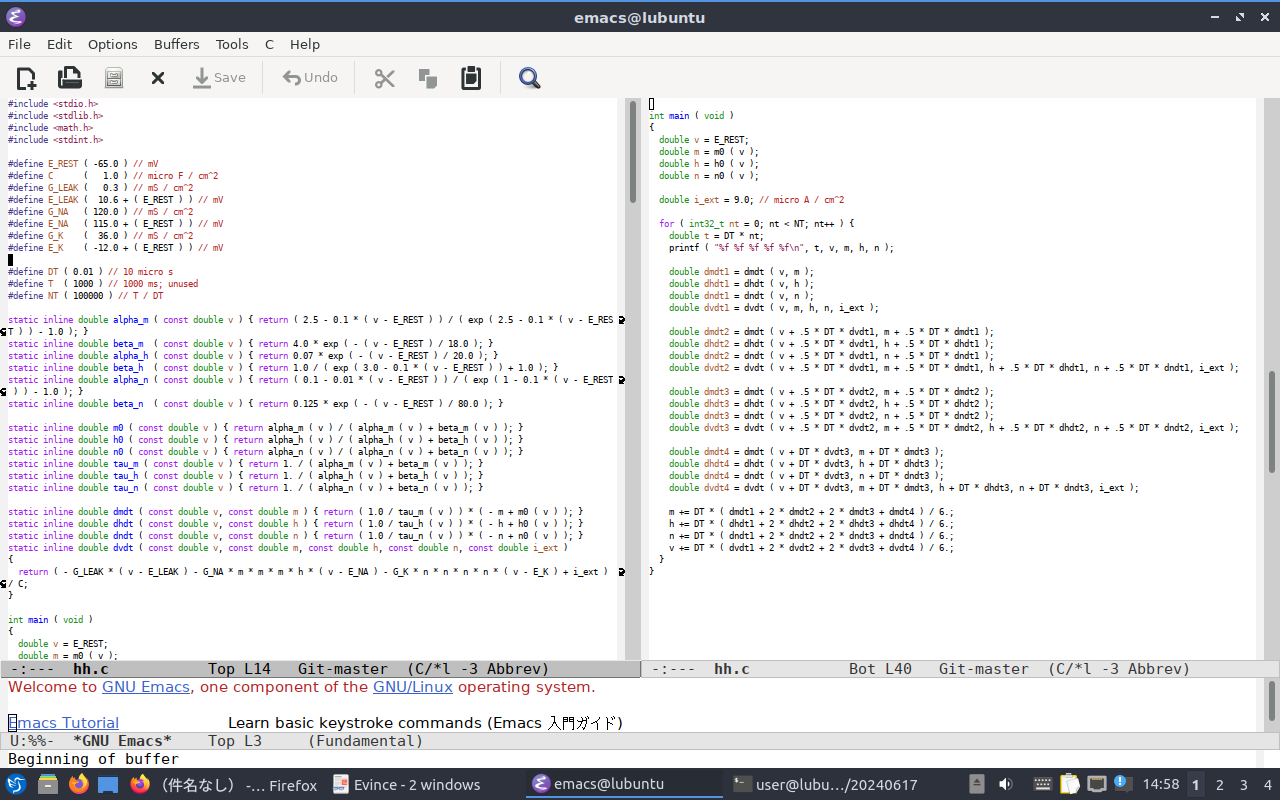
\includegraphics[width=0.5\textwidth]{images/hh_code.png}
    \caption{hh.c}
\end{figure}

\begin{figure}[h]
    \centering
    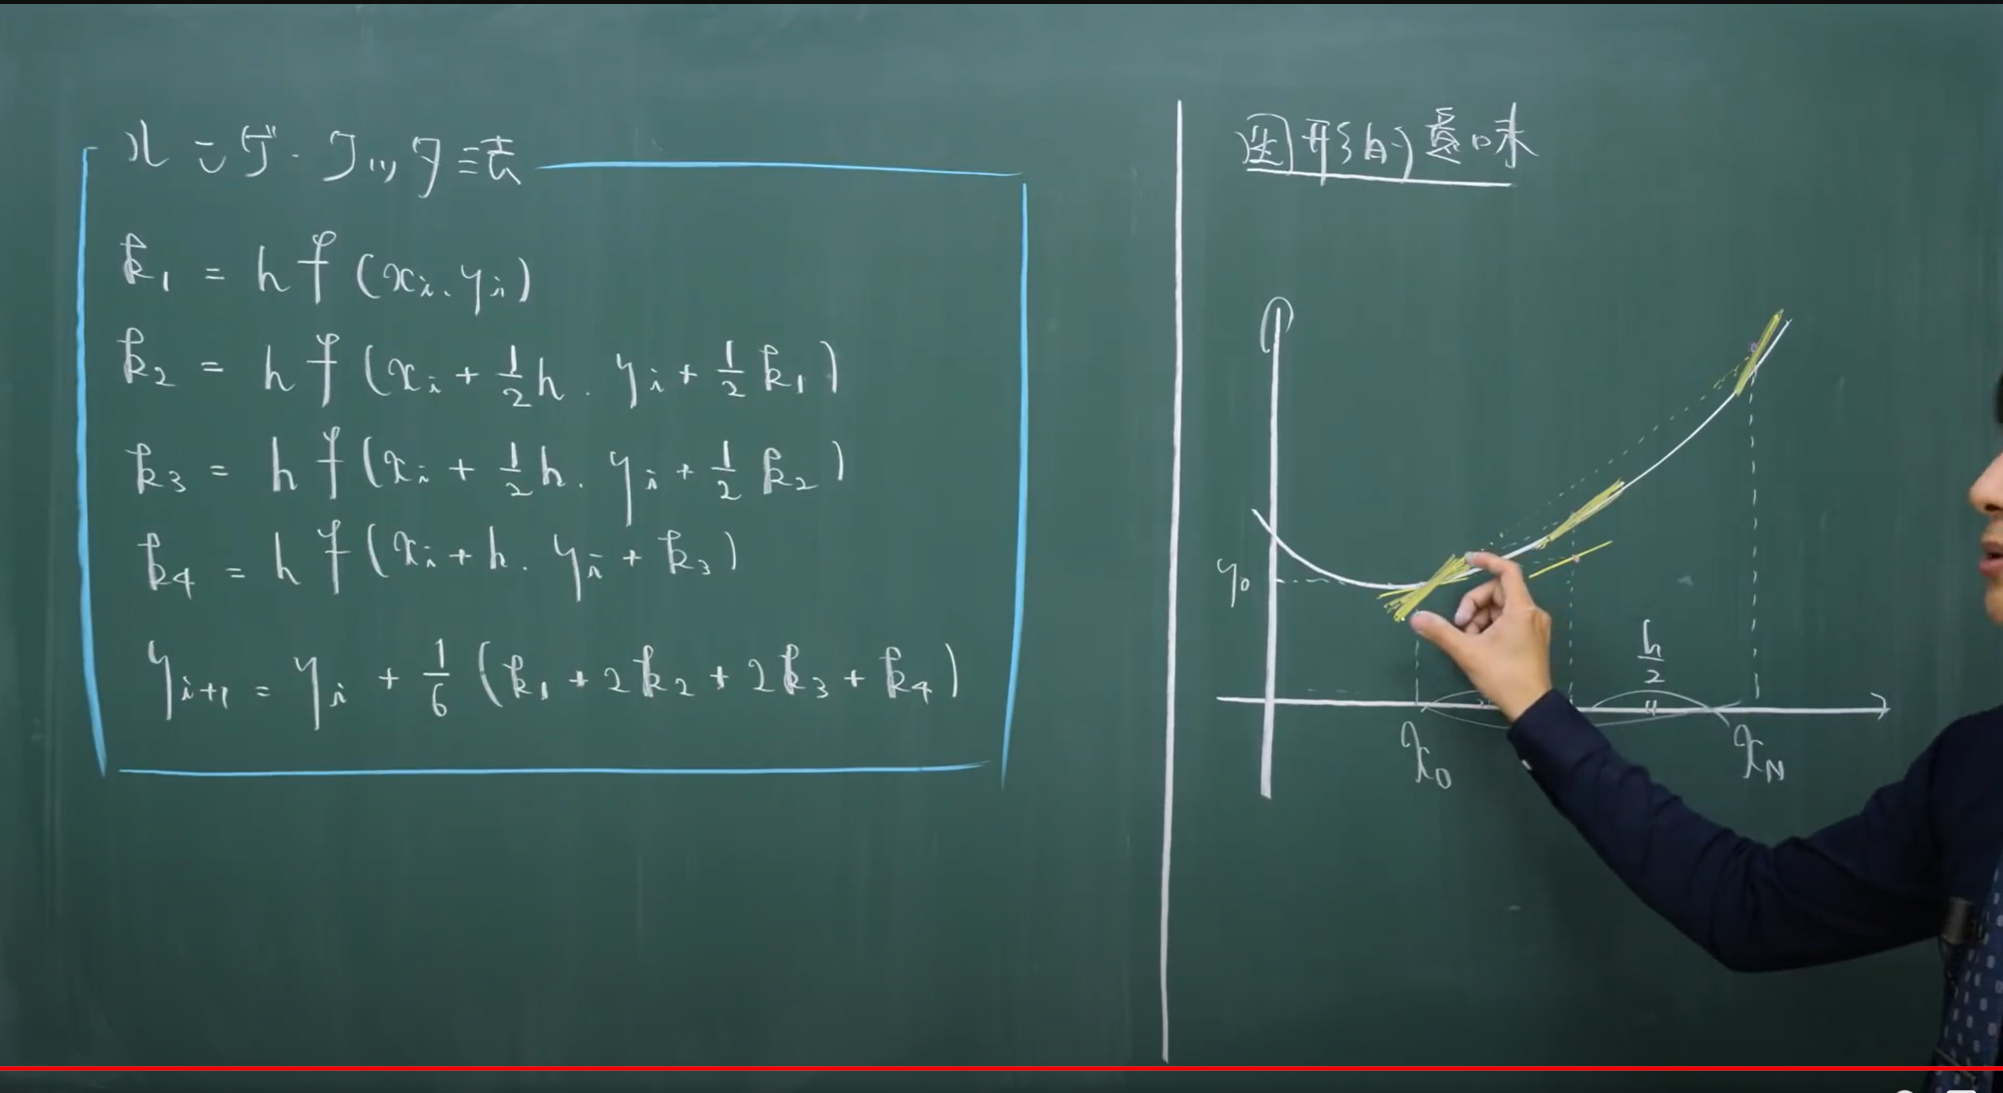
\includegraphics[width=0.5\textwidth]{images/rk4.png}
    \caption{(4次)ルンゲクッタ法}
\end{figure}

\begin{figure}[h]
    \centering
    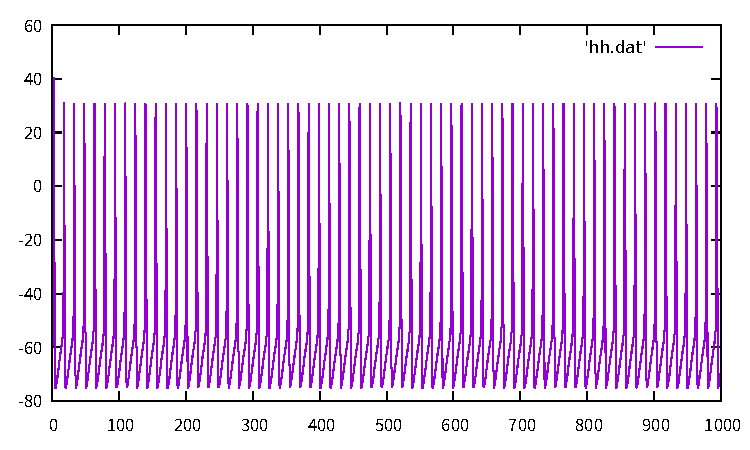
\includegraphics[width=0.5\textwidth]{images/0301_hh_1000.pdf}
    \caption{1000ms間の計算結果}
\end{figure}

\begin{figure}[h]
    \centering
    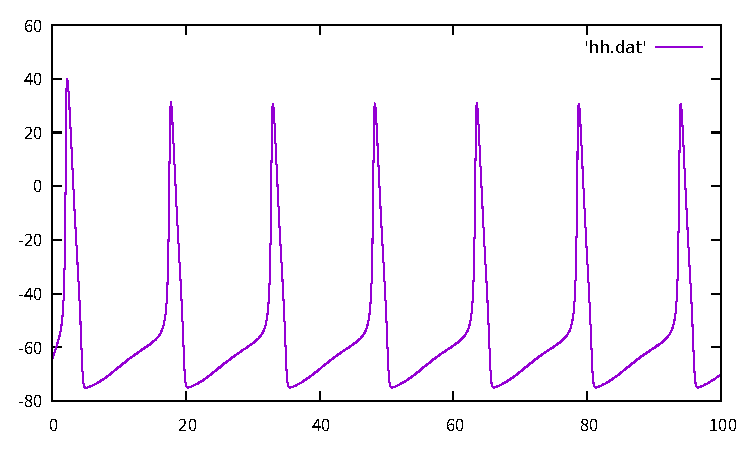
\includegraphics[width=0.5\textwidth]{images/0301_hh_100.pdf}
    \caption{先頭100ms間の拡大図}
\end{figure}


\vspace{\baselineskip}

このプログラムにおいては$T=1000[\mathrm{ms}]$間の計算を,時間刻み幅$\delta t=10 [\mu \mathrm{s}]$で計算している.

また外部電流(細胞の外部から注入する電流)$I_{\mathrm{ext}}(t)$は$9.0[\mu \mathrm{A} / \mathrm{cm}^2$にセットする.
結果が示すように,外部電流を加え続けると,ニューロンは持続的にスパイクを発射する.そこで,ごく短い時間,例えば$1[\mathrm{ms}]$だけ電流を加えるようにしてみると,スパイクは一回のみ発射される.


\begin{figure}[h]
    \centering
    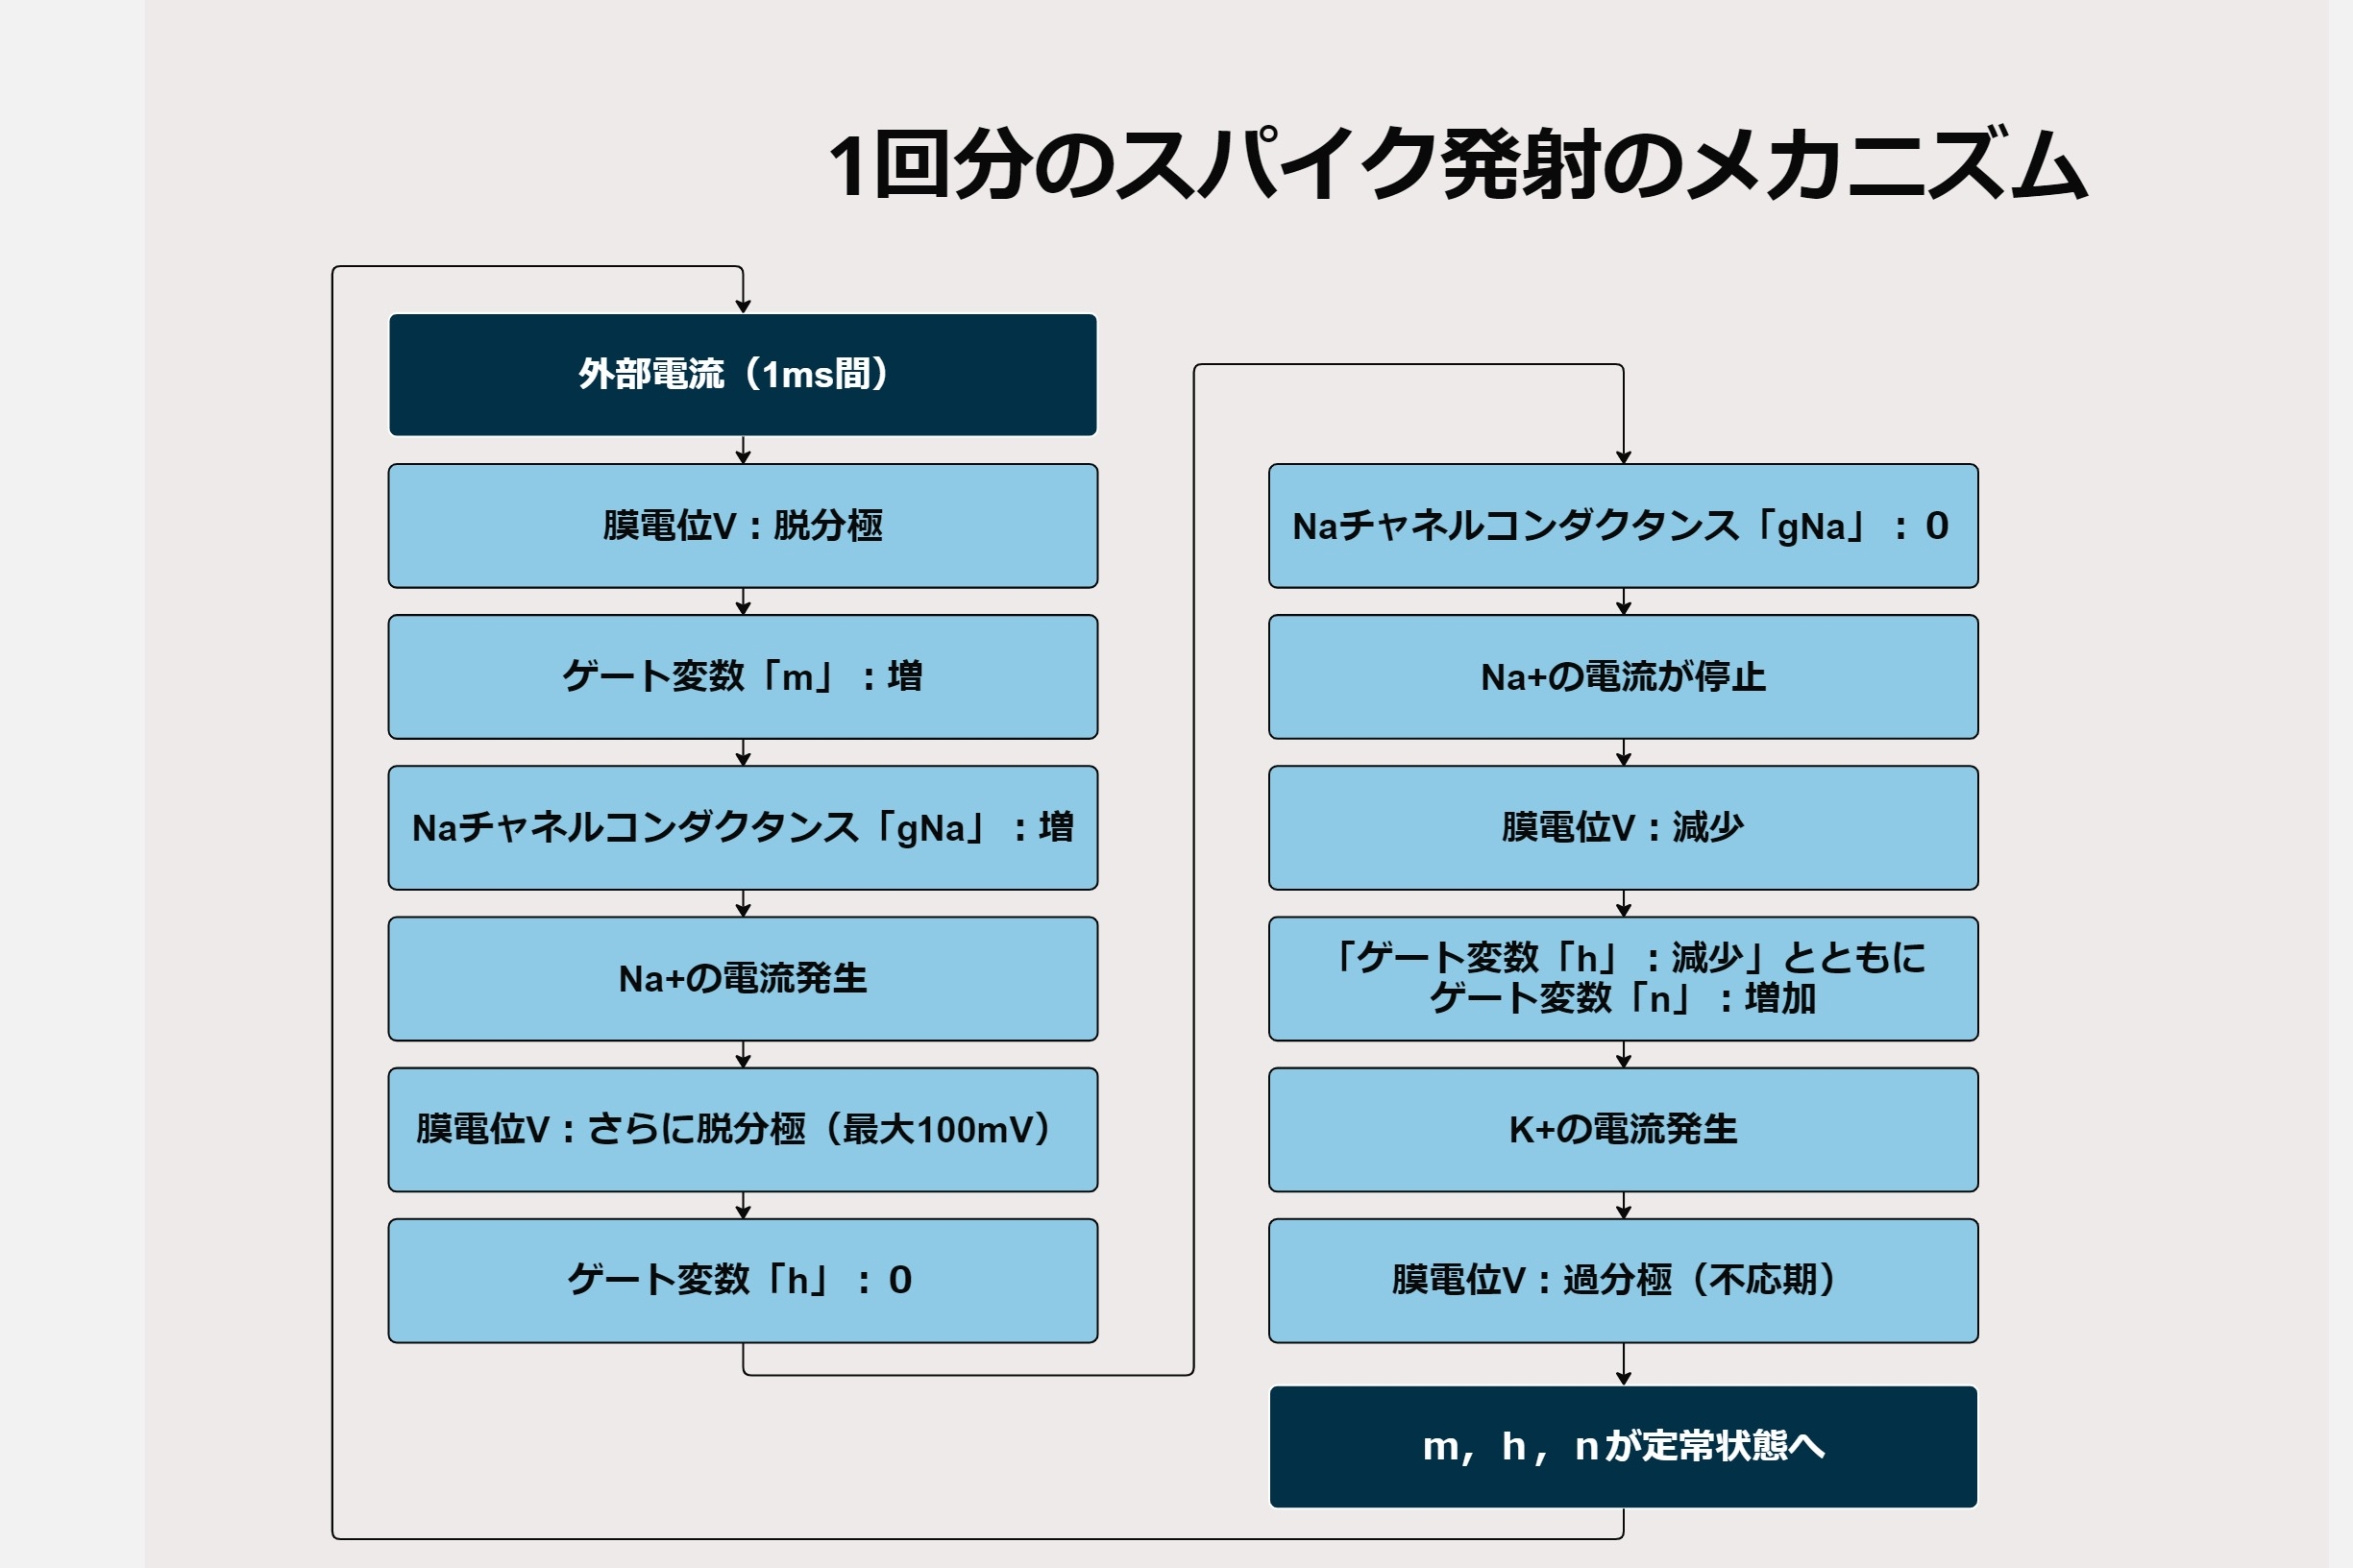
\includegraphics[width=0.5\textwidth]{images/flow.jpg}
    \caption{スパイクの一回の発射の流れ}
\end{figure}


\begin{figure}[h]
    \centering
    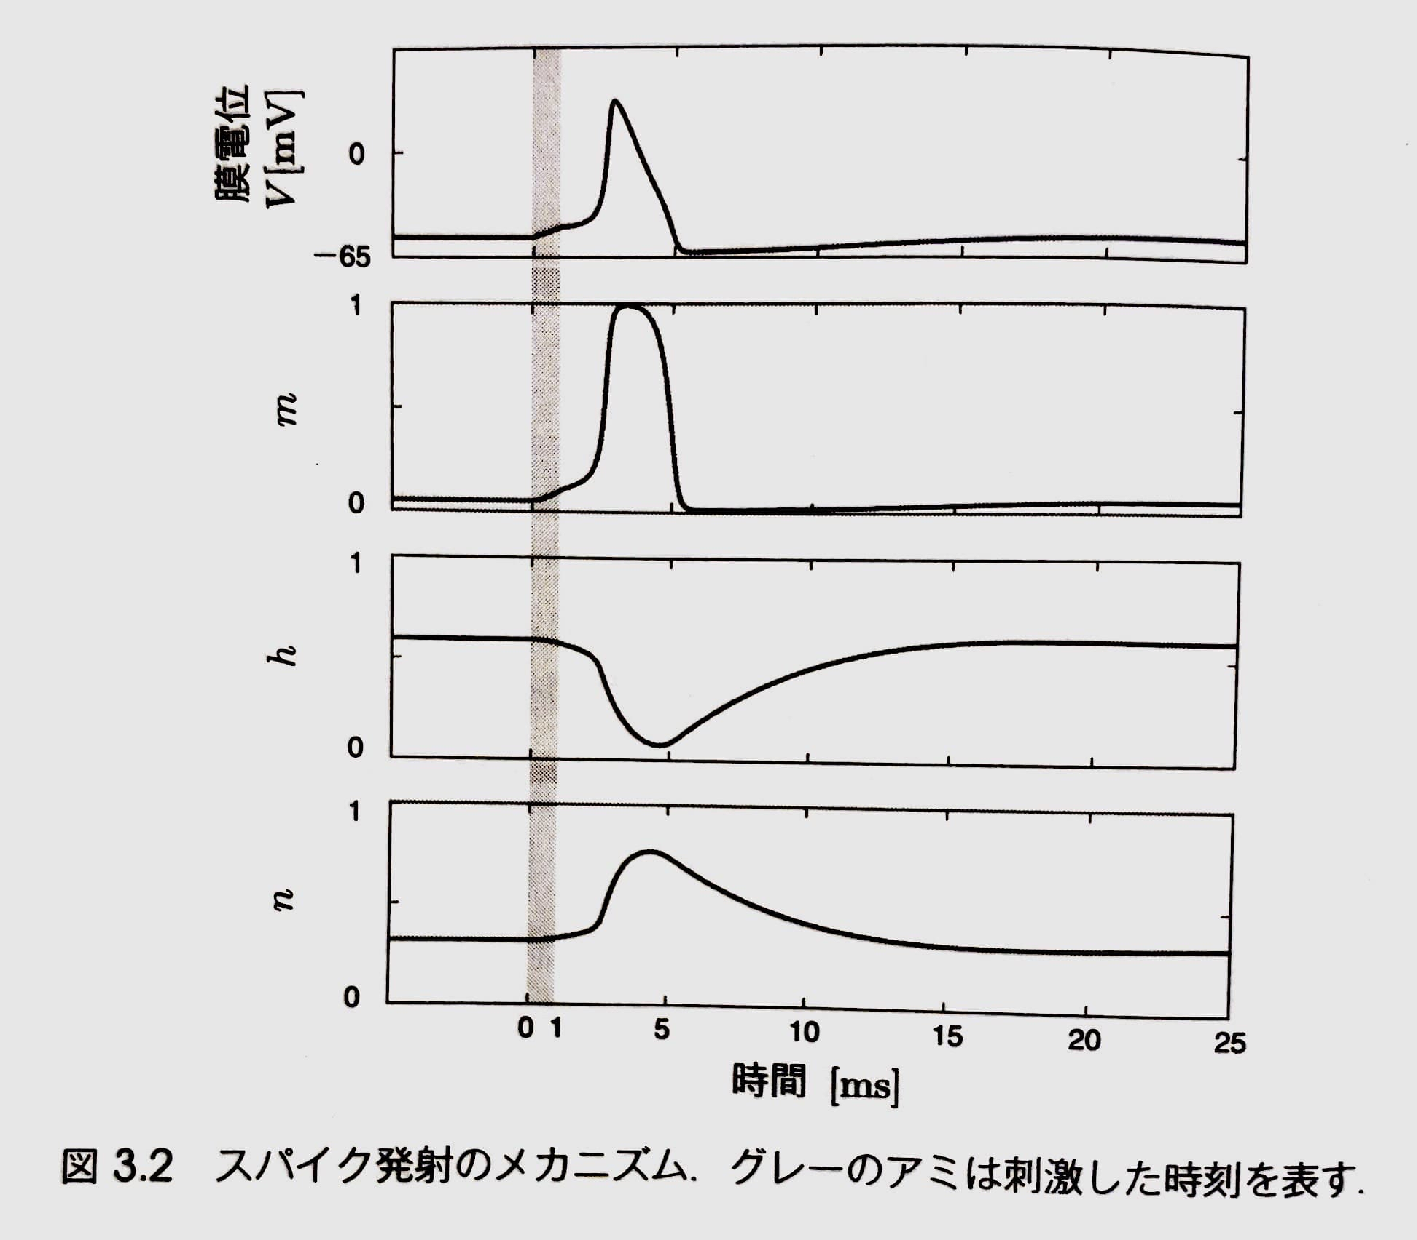
\includegraphics[width=0.5\textwidth]{images/spike1.pdf}
    \caption{スパイクの一回の発射の波形とゲート変数(m,h,n)の波形}
\end{figure}


外部電流の強度が高まるほど,スパイクの発火頻度は上昇する.このような,外部電流がある値を超えると突然高頻度でスパイクを発射するニューロンをType \romannumeral 2 ニューロンと呼ぶ.




\subsubsection*{3.1.4 HHモデルの拡張}

\begin{figure}[h]
    \centering
    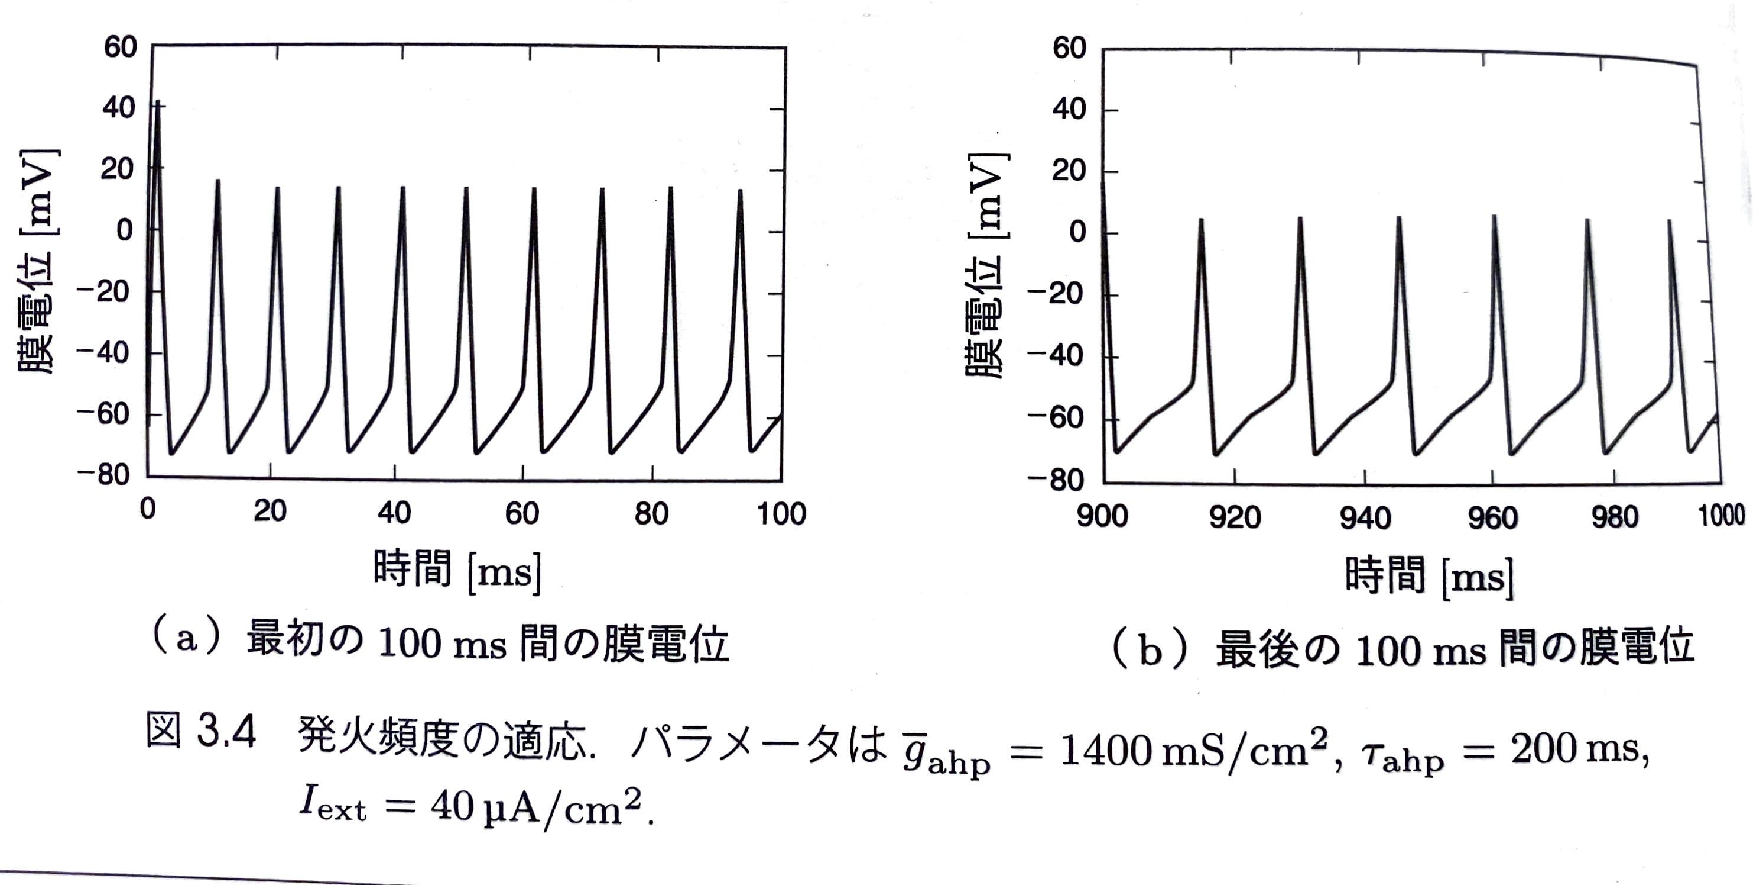
\includegraphics[width=0.5\textwidth]{images/tekio.pdf}
\end{figure}
先に示したHHモデルにおいては,発火頻度は一定のままであったが,実際のニューロンにおいては発火頻度は次第に減少する.この現象を適応と呼ぶ.適応は後過分極電流$I_{ahp}(t)$に起因する.

また,Type \romannumeral 2ニューロンに対して,外部電流に比例して連続的に発火頻度が上昇していくニューロンをType \romannumeral 1ニューロンと呼び,大脳皮質のニューロンなどがこれに当たる.また,ニューラルネットワークで実装されるニューロンもこのような挙動をとる.
\begin{figure}[h]
    \centering
    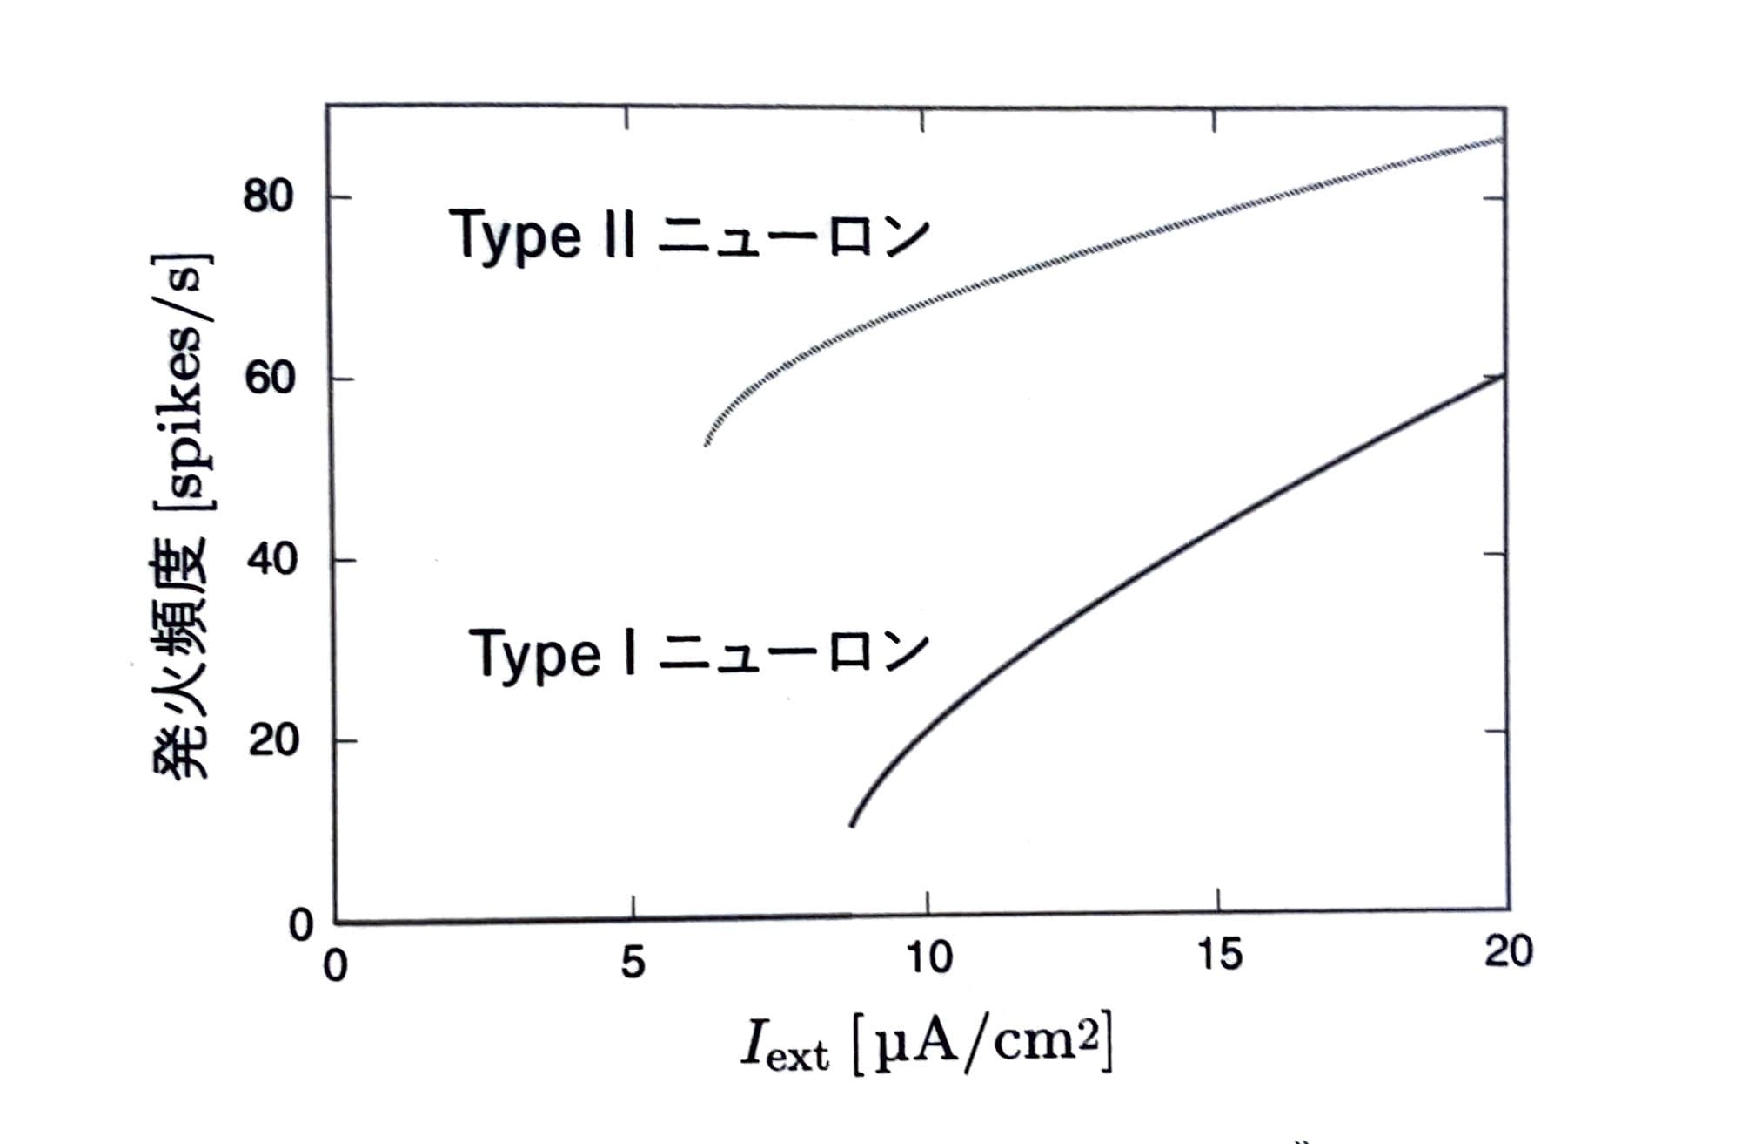
\includegraphics[width=0.5\textwidth]{images/i_f_.pdf}
    \caption{Type \romannumeral 1ニューロン,Type \romannumeral 2ニューロンのI-Fカーブ}
\end{figure}
Type \romannumeral 1ニューロンを得る方法として,$K^{+}$イオンの過渡電流を加えることが挙げられる.\footnote{$K^{+}のかと電流を考慮したモデルとしてコナー・スティーブンスモデルがある.$}これにより膜が過分極され,スパイク発射が遅延して発火頻度が減少する.

\vspace{\baselineskip}
\vspace{\baselineskip}

\subsection*{3.2 積分発火型モデルのシミュレーション}
\subsubsection*{3.2.1 積分発火型モデル}

HHモデルは,実際のニューロンのメカニズムに忠実な分,
\begin{itemize}
 \item V,m,h,nと,変数を4つも用いる
 \item スパイクが素早いダイナミクスを取る為,刻み幅を小さく取る必要がある
\end{itemize}

といった問題がある.脳の情報処理において重要なのはスパイクの発火頻度やタイミングにあり,スパイクの波形自体には情報はないと考えられている.そのような前提に立った上で,1変数のみを用い,刻み幅を比較的粗くとれるシンプルなニューロンモデルとして,積分発火型(Leaky Integrate-and-Fire, LIF)モデルがある.

\vspace{\baselineskip}
\vspace{\baselineskip}

\section{Letter:Interspike Interval Statistics in the Stochastic Hodgkin-Huxley Model: Coexistence of Gamma Frequency Bursts and Highly Irregular Firing(確率的Hogkin-Huxleyモデルにおけるスパイク間隔統計・ガンマ周波数バーストと高い不規則発火の共存)}
\subsection{概要}
HH方程式をNa/Kチャネルのノイズと定常電流をシミュレーションすると,スパイク間隔の分布は二峰性を示す.
\begin{itemize}
 \item 通常仮定される指数的な尾部
 \item 短いスパイク間隔値に中心を置く狭いガウスピーク
\end{itemize}
一般的なニューロンにおいてもこの二峰性ISI(スパイク間間隔)分布を持っており,Type \romannumeral 2 発火を持つニューロンの有用なモデルになる可能性がある.この性質の(?)基礎となるメカニズムは以下による.
\begin{itemize}
 \item a subcritical Hopf bifurcation(亜臨界ホップ分岐?)
 \item a switching region in phase-space where a fixed point is ery close to a system limit cycle(固定点がシステムのリミットサイクルに非常に近い位相空間内の切り替え領域?)
\end{itemize}

このようなメカニズムは多くの異なるクラスのニューロンに存在し,広く観察される高い不規則なスパイクに寄与している可能性がある.

\subsection{導入}
\subsubsection{スパイクタイムの変動性の要因 - チャネルノイズ}
同一の入力に対するスパイクタイムの変動性の一つの説明として,シナプスノイズ\footnote{シナプス応答の不規則な変動}が挙げられるが,別の要因として確率的イオンチャネル活動(?)からのノイズがあり,これが神経閾値(?)とスパイクタイムの信頼性に影響を与えている可能性がある.実際,特定の小さなニューロンにおいて,単一チャネルの開口が活動電位を引き起こすことがある.

\vspace{\baselineskip}
この書面では,HH方程式で記述された単一ニューロンが,ISI(スパイク間間隔)の特徴的な二峰性分布(指数的な尾部/最短間隔におけるガウスピーク)を持つスパイクタイム変動性を生み出すことを示す.

\subsubsection{二峰性を示すニューロン}
この,最初のピークの位置がガンマ周波数帯域(40~100Hz)に見られるような二峰性分布は,実際のニューロンの観察においても,HHモデルにおいても観察される.HHモデルは,コンダクタンスを陽に記述する「コンダクタンスベースモデル」である.一方で,積分発火型モデルのような簡易的なモデルにおいては,コンダクタンスが式中に存在しない「カレントベースモデル」である.

\vspace{\baselineskip}
多くのニューロンは,HHモデルと同一のType \romannumeral 2に分類され,段階的に増加する外部電流に対し,正(非零)の頻度でスパイクを開始する.このType \romannumeral 2の挙動は,a subcritical Hops bifurcation(亜臨界ホップ分岐???)の存在により生じる.

\vspace{\baselineskip}
HHモデルは4変数のシステムで,それを2変数に簡約したモデルが多く提案されており,その一つがフィッシュフュー南雲(FitHugh-Nagumo)方程式である.他に,Morris-Lecarモデルは,フジツボなどの甲殻類の$Ca^{+}$,$K^{+}$チャネルを持つモデル(=コンダクタンスベースモデル)である.このような2変数のモデルを用いて,HHモデルに見られるようなISIの二峰性分布の動的説明を試み,固有のチャネルノイズの影響によって,不規則なハッカとガンマ周波数のバーストが組み合わされてることを示す.
\vspace{\baselineskip}

\subsection{Methods - 研究方法(割愛)}
\vspace{\baselineskip}

\subsection{Results - 結果}
ISIを周波数ヒストグラムにプロットすると,2つピークが確認できる.入力電流$3\mu \mathrm{A}$に対して,入力電流$0\mu \mathrm{A}$における2番目のピークは相対的にほとんど目立っていない.このことから,様々な入力電流に対して周波数ヒストグラムをプロットすることが提案された.結果,2番目のピークは入力電流と線形的に増加する結果が得られた.

\begin{figure}[h]
    \centering
    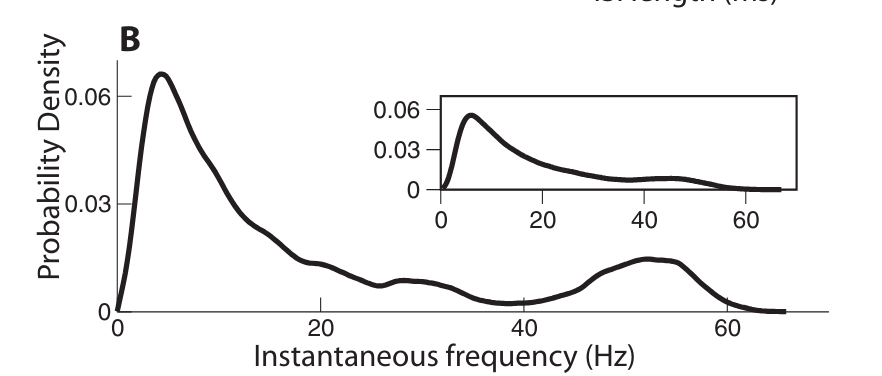
\includegraphics[width=0.5\textwidth]{images/frequency_3.png}
    \caption{入力電流3と0$\mu \mathrm{A}$における周波数ヒストグラム}
\end{figure}


\begin{figure}[h]
    \centering
    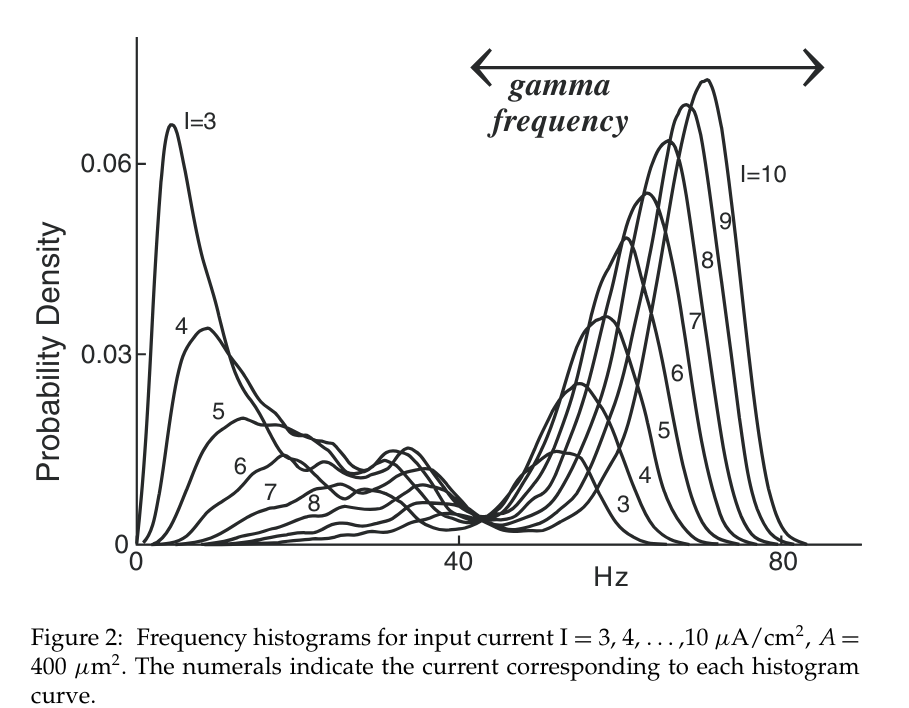
\includegraphics[width=0.5\textwidth]{images/frequency_i.png}
    \caption{様々な入力電流における周波数ヒストグラム}
\end{figure}




\vspace{\baselineskip}
\vspace{\baselineskip}



\section{今週やること}
\begin{itemize}
 \item HHモデルを簡易化したモデル(積分発火型モデル等)のメカニズムの学習
 \item 研究テーマ(ガウスノイズ?)関連の先行研究のサーチ
\end{itemize}




\begin{thebibliography}{99}
% \bibitem{lite1} 和田勝 ``筋肉による筋収縮の司令'' 生命科学C, 2001, https://www.tmd.ac.jp/artsci/biol/textlife/neuron.html.
% \bibitem{lite2} R. Hosaka, T. Kimura, and T. Matsuura, ``title,'' journal name, pp.10-20, 2021.
\bibitem{lite2} ???, ``Interspike Interval Statistics in the Stochastic Hodgkin-Huxley Model: Coexistence of Gamma Frequency Bursts and Highly Irregular Firing(確率的Hogkin-Huxleyモデルにおけるスパイク間隔統計・ガンマ周波数バーストと高い不規則発火の共存)'' MIT Press Direct, 2007, https://direct.mit.edu/neco/article/19/5/1215/7185/Interspike-Interval-Statistics-in-the-Stochastic
\end{thebibliography}
\end{document}
